% !TeX encoding = UTF-8
\documentclass[12pt]{article}

%%% 
\usepackage{hyperref}

\usepackage{amsmath} 
\usepackage{amssymb}
\usepackage{amsfonts}
\usepackage{amsthm}
\usepackage{graphicx}
\usepackage{xcolor}

\textwidth 175mm \textheight 230mm \topmargin -10mm \oddsidemargin
-5mm


%%% Теоремы и утверждения
\newtheorem{proposition}{Proposition}
\newtheorem{lemma}{Lemma}
\newtheorem{theorem}{Theorem}
\newtheorem{definition}{Definition}
\newtheorem{corollary}{Corollary}

\theoremstyle{definition}
\newtheorem*{demo}{Proof}
\newtheorem{remark}{Remark}

%%% Свои операторы
\newcommand\Tr{\operatorname{Tr}}
\newcommand\tr{\operatorname{tr}}
\newcommand\diag{\operatorname{diag}}

\renewcommand\Re{\operatorname{Re}}
\renewcommand\Im{\operatorname{Im}}


\newcommand\bra{\left<}
\newcommand\ket{\right>}
\newcommand{\braket}[1]{\bra#1\ket}
\newcommand{\mf}[1]{\mathfrak{#1}}

\def\al {\alpha}
\def\be {\beta}
\def\br {{\Bbb R}}
\def\bc {{\Bbb C}}
\def\const{\hbox{\rm const}}

\def\de {\delta}
\def\DE {\Delta}
\def\e {\eta}
\def\f {\frac}
\def\ga {\gamma}
\def\GA {\Gamma}
\def\intl {\int\limits}
\def\la {\lambda}
\def\LA {\Lambda}
\def\liml {\lim\limits}
\def\om {\omega}
\def\OM {\Omega}
\def\OB {\ov B}
\def\pr {\partial}
\def\sg {\sigma}
\def\tl {\tilde}
\def\ve {\varepsilon}
\def\vp {\varphi}
\def\th {\theta}
\def\Bbb{\mathbb}

\begin{document}
		\begin{center}
		\Large
		\textbf{Gaussian ansatz}
		
		\large 
		\textbf{K.Sh. Meretukov}\footnote{Faculty of Physics, Lomonosov Moscow State University, Leninskie Gory, Moscow 119991, Russia\\
			E-mail:\href{mailto:meretukov.khazret@gmail.com}{meretukov.khazret@gmail.com}}
		\textbf{A.E. Teretenkov}\footnote{Department of Mathematical Methods for Quantum Technologies, Steklov Mathematical Institute of Russian Academy of Sciences, ul. Gubkina 8, Moscow 119991, Russia\\ E-mail:\href{mailto:taemsu@mail.ru}{taemsu@mail.ru}}
		\\[1mm]
	\end{center}
	
	\footnotesize
	
	\normalsize
	
	\section{\label{sec:introduction}Introduction}
	
	Recently, the study of systems with Kerr nonlinearity has become a popular problem \cite{KerrIntr}. Also, recently there has been increasing interest in approximations by Gaussian ansatz in other fields, such as quantum spin chain theory, the method we develop may be useful in these fields as well \cite{GaussState}. Also this approach allows to consider not only those cases when at zero order the dynamics is described by a Gaussian channel, but also to consider non-Gaussian channels in real physical systems as nonlinear, but Gaussian channels. This peculiarity is useful in quantum theory of information, since many properties of Gaussian channels are known \cite{Kholevo}.
	
	However, when considering the Kerr model, there is a problem with the solution when the number of particles is large \cite{MaslovN}. One of the solution methods is the solution by means of classical stochasticity, but in this case all quantum effects are lost \cite{MaslovSolve}. Our method is not limited in dissociation of a small number of particles and can work for any number of particles.
	
	\section{\label{sec:GeneralApproch}General projection approach for Gaussian approximation and systematic corrections to it}
	
	Let's introduce some notations that will help to simplify the writing of some expressions.
	
	Let us introduce $\mf{a} = (a_1, a_2, \ldots, a_N, a_1^+, a_2^+,\ldots,a_N^+)^T$. Then an arbitrary quadratic form on the birth and annihilation operators can be written as $\dfrac{1}{2}\mf{a}^TK\mf{a} + g^T\mf{a}$, where $K \in \mathbb{C}^{2N \times 2N}, g \in \mathbb{C}^{2N}$. Then the commutation relations are written in the form 
	
	\begin{equation}
		\label{eq:ComRel}
		[f^T\mf{a},\mf{a}^Tg] = -f^TJg,
	\end{equation}
	where $f \in \mathbb{C}^{2N}, g \in \mathbb{C}^{2N}$ and the matrix $J$ has the form
	
	\begin{equation*}
		J = \begin{pmatrix}
			0 & -I_N \\
			I_N & 0
		\end{pmatrix},
	\end{equation*}
	where $I_N$ is a unit matrix.
	
	\begin{equation*}
		E = \begin{pmatrix}
			0 & I_N \\
			I_N & 0
		\end{pmatrix}.
	\end{equation*}
	
	\begin{equation*}
		I = \begin{pmatrix}
			I_N & 0 \\
			0 & I_N
		\end{pmatrix}.
	\end{equation*}
	
	Also such notations allow to write the following expressions compactly
	
	\begin{equation*}
		\operatorname{tr} \mathfrak{a}^T f g^T  \mathfrak{a} \rho =   f^T \operatorname{tr}(\mathfrak{a}  \mathfrak{a}^T \rho) g = f^T D g = \Tr D g  f^T  = \Tr f g^T D^T
	\end{equation*}
	hence 
	\begin{equation}
		\label{eq:CompFormOfAv}
		\operatorname{tr} \mathfrak{a}^TA \mathfrak{a} \rho  = \Tr AD^T
	\end{equation}
	
	
%	\section{\label{sec:QuadraticForm} Quadratic form}
	The Gaussian ansatz is used in this paper 
	
	\begin{equation}
		\label{eq:ProjForAv}
		\rho_{anz}=\exp(\dfrac{1}{2}\mathfrak{a}^TK\mathfrak{a} + g^T\mathfrak{a} + s),
	\end{equation}
	where $e^s = \sqrt{|det(e^{KJ} - I)|}e^{\frac{1}{2}g^TK^{-1}g}$.
	
	The characteristic function of such ansatz has the form
	
	\begin{equation}
		\chi(\textbf{z}) = \Tr(\rho_{anz} e^{\textbf{z}^T\mathfrak{a}}) =  e^{\frac{1}{2}(i\textbf{z}^T)C(i\textbf{z}) + i\textbf{z}^Tm}
	\end{equation}
	
	Let's write out some of the beneficial properties of such ansatz.
	
	\begin{theorem}
		\label{th:KvFor}
		\begin{align*}
			\label{eq:KvFor}
			e^{\dfrac{1}{2}\mf{a}^TK\mf{a} + g^T\mf{a}}(\dfrac{1}{2}\mf{a}^TM\mf{a} + f^T\mf{a})e^{-(\dfrac{1}{2}\mf{a}^TK\mf{a} + g^T\mf{a})} &= \dfrac{1}{2}\mf{a}^Te^{-KJ}Me^{JK}\mf{a} + \left(e^{-kJ}M\dfrac{e^{JK}-I}{JK}Jg + e^{-KJ}f\right)^T\mf{a} + \nonumber\\
			&+ \left(\dfrac{1}{2}g^TJ\dfrac{e^{-KJ}-I}{KJ}M + f^T\right)\dfrac{e^{JK} - I}{JK}Jg&
		\end{align*}
	\end{theorem}
	\begin{demo}
		The proof can be found in \cite{Dis}. 
	\end{demo}
	
	This feature allows us to carry the density matrix through the quadratic form of the birth/annihilation operators.
	
	However, the main feature that is the reason we use the Gaussian ansatz is Wick's theorem.
	
	\begin{theorem}
		\label{th:IW0}
		For a Gaussian ansatz with zero mean and with the matrix of second moments $D$ it follows that 
		\begin{equation*}
			\braket{\mf{a}_I} = \sum\limits_{I = I_1 \sqcup I_2}\mu_{I_1}D_{I_2}.
		\end{equation*}
	\end{theorem}
	\begin{demo}
		The proof of this theorem and more details can be found in \cite{NosalTeretenkov}
	\end{demo}
	

	
	
%	\section{\label{sec:ProjOper} Projection operator}
	
	In this paper, we use a projective operator on Gaussian ansatzians. That is, we consider such operators $\mathcal{P}$ which
	
	\begin{align*}
		\mathcal{P}^2(t)& = \mathcal{P}(t), \\
		\mathcal{P}\rho(t)& = \rho_{rel}(t) = \exp(\dfrac{1}{2}\mathfrak{a}^TK\mathfrak{a} + g^T\mathfrak{a} + s).
	\end{align*}
	
	Using such a projector, it can be shown that for the $\ref{eq:EvEq}$ system in the weak coupling limit $\la \rightarrow 0$ the following equation is fulfilled
	
	\begin{align}
		&\frac{d}{dt} \vec{E}(t) = \lambda   \Tr ( \vec{P}\mathcal{L}(t)\rho_{ans} (\vec{E}(t) ) + \lambda^2 \Tr \left( \vec{P} \mathcal{L}(t)  \int_{t_0}^t dt_1 \mathcal{L}(t_1)\rho_{ans} (\vec{E}(t))   \right) \nonumber \\
		& 	-  \lambda^2 \Tr\Biggl( \vec{P} \left(\Tr (  \vec{P} \mathcal{L}(t)\rho_{ans} (\vec{E}) ) , \frac{\partial \rho_{ans}(\vec{E})}{\partial \vec{E}} \right) \times \nonumber\\
		& \qquad \times \left(\Tr (  \vec{P}\int_{t_0}^t dt_1\mathcal{L}(t_1)\rho_{ans} (\vec{E}) )  , \frac{\partial \rho_{ans}(\vec{E})}{\partial \vec{E}} \right) \Biggr)_{\vec{E} =\vec{E}(t) }. \label{eq:secOrderEqE}
	\end{align}
	where $\vec{E}(t) = \Tr\rho(t)\vec{P}$.
	
	As can be seen, the first order coincides with the equation in the Heisenberg representation.
	
	The equation \ref{eq:secOrderEqE} is written in the interaction representation, thus we need to move into this representation. Then
	
	\begin{equation}
		\label{eq:IntRepRho}
		\rho(t) \equiv e^{-\mathcal{L}_0t}\rho_{ans}(t).
	\end{equation}
	
	Then the density matrix \ref{eq:IntRepRho} satisfies the equation 
	
	\begin{equation}
		\label{eq:MainEq}
		\dfrac{d}{dt}\rho(t) = \la\mathcal{L}(t)\rho(t),
	\end{equation}
	where
	\begin{equation}
		\label{eq:IntRepL}
		\mathcal{L}(t) = e^{-\mathcal{L}_0t}\mathcal{L}_ie^{\mathcal{L}_0t}
	\end{equation}
	
	In order to find the generator in the interaction representation we need to solve equation
	
	\begin{equation}
		\label{eq:InteractionReprSuper}
		\dfrac{d}{dt}\mathfrak{L}(t) = -J_2L_t\mathfrak{L}-J_2F,
	\end{equation}
	where $\mf{L}$ is a superoperator of the following form
	
	\begin{equation*}
		\mathfrak{L} = (\mathfrak{a}\cdot,\cdot E\mathfrak{a})^T
	\end{equation*}
	
	Since in our case all coefficients do not depend on time, it follows that the solution of this equation is the function
	
	\begin{equation}
		\label{eq:SolOfSuper}
		\mathfrak{L}(t) = L^{-1}e^{-LJt}L\mf{L}(0) + L^{-1}(e^{-LJt} - I)F
	\end{equation}
	
	
	Then, if we want to find $[a^+a^+aa,\cdot](t)$ we need to calculate the expression
	
	\begin{equation*}
		\mathfrak{L}_2\mathfrak{L}_2\mathfrak{L}_1\mathfrak{L}_1 - \mathfrak{L}_4\mathfrak{L}_4\mathfrak{L}_3\mathfrak{L}_3,
	\end{equation*}
	where the expression $\mathfrak{L}_i$ implies the $i$-th row of the corresponding vector $\mathfrak{L}$.
	
	
	
	Equation \ref{eq:secOrderEqE} contains the ansatz derivative. In order to obtain an explicit form of this derivative we need to find the relationship between the matrix $K$ and the covariance matrix $C$.
	
	\begin{equation}
		\label{eq:ConOfCFromK}
		C = -\frac{J}{2}\text{coth}\left(\frac{KJ}{2}\right),
	\end{equation}
	expressing $K$ from this equation, we obtain
	
	\begin{equation}
		\label{eq:ConOfKFromC}
		KJ = 2\text{arcoth}\left(-2J^{-1}C\right).		
	\end{equation}
	
	The derivative of the Gaussian exponent can be expressed as a quadratic form
	
	\begin{equation}
		\label{eq:DerWithLin}
		\frac{d}{dt}\rho_{anz} = (\frac{1}{2}\mf{a}^TM\mf{a} + \mf{a}^TG + c)\rho_{anz},
	\end{equation}
	where
	\begin{align*}
		M &= \frac{I}{C - \frac{J}{2}}\left(\frac{d}{dt}C\right)\frac{I}{C + \frac{J}{2}},\\
		G &= \left(  I + \frac{2I}{2J^{-1}C - I}  \right)\frac{d}{dt}\left(\frac{I}{C + \frac{J}{2}}m\right),\\
		c &=-m^T\frac{I}{2J^{-1}C -  I}\frac{d}{dt}\left(\frac{I}{C + \frac{J}{2}}m\right) + \frac{1}{2}\frac{d}{dt}m^T\left( \frac{I}{2J^{-1}C - I} - \frac{I}{2J^{-1}C + I} - KJ \right)J^{-1}m + \frac{d}{dt}c_t,
	\end{align*}
	where $g = -Km$, in which $m = (\braket{a} , \braket{a^+})^T$ and $C$ --- covariance matrix.
	
	A detailed derivation is provided in the appendix \ref{App}.
	
	The formula for the derivative of Gaussian ansatz can be found in \cite{Dis}.
	
	\begin{equation}
		\label{eq:difofrho}
		\left(\dfrac{d}{dt}e^{\frac{1}{2}\mathfrak{a}^TK\mathfrak{a} + c}\right)e^{-\frac{1}{2}\mathfrak{a}^TK\mathfrak{a} - c} = \dfrac{1}{2}\mathfrak{a}^Te^{-KJ}\dfrac{d}{dt}e^{KJ}J^{-1}\mathfrak{a} + \dfrac{d}{dt}c,
	\end{equation}

	

	
	However, in fact in Equation 11 we have this expression squared, in order to get the desired degeneracy the density matrix has to be carried through the quadratic form, i.e.
	
	\begin{equation}
		\label{eq:DenMatrOverForm}
		\rho_{anz}(\frac{1}{2}\mf{a}^TM\mf{a} + f^T\mf{a} + c) = (\mf{a}^TM'\mf{a} + f'^T\mf{a} + c')\rho_{anz},
	\end{equation}
	where
	\begin{align*}
		M' &= \frac{1}{2}e^{-KJ}Me^{JK}, \\
		f' &= e^{-KJ}M\frac{e^{JK} - I}{JK}Jg + e^{-KJ}f, \\
		c' &= \left( \frac{1}{2}g^TJ\frac{e^{-KJ} - I}{KJ}M +f^T  \right)\frac{e^{JK} - I}{JK}Jg + c.
	\end{align*}
	
	Using the relationship between matrices $K$ and $C$ these expressions can be simplified. As a result, we obtain
	
	\begin{align}
		\label{eq:mfcdot}
		M' &= \frac{1}{2}\left(I + \frac{2I}{2J^{-1}C - I}\right)MJ\left(I - \frac{2I}{2J^{-1}C + I}\right)J^{-1}, \nonumber\\
		f' &= 2\left(I + \frac{2I}{2J^{-1}C - I}\right)MJ\frac{I}{2J^{-1}C + I}J^{-1}m + \left(I + \frac{2I}{2J^{-1}C - I}\right)f, \\
		c' &= 2\left(f^T - m^T\frac{I}{2J^{-1}C - I}M\right)J\frac{I}{2J^{-1}C + I}J^{-1}m + c
	\end{align}
	
	We also need to find a renormalisation for the ansatz square. 
	
	\begin{equation}
		\label{eq:RhoSq}
		\rho_{0,C}^2 = \frac{1}{\sqrt{|\det(2 C)|}} \rho_{0,C'}.
	\end{equation}
	where 
	\begin{equation*}
		C' = - \frac{J}{4}\left(\frac{1}{2 J C} + 2 J C\right).
	\end{equation*}
	
	The derivation of this relation can be seen in \ref{App}
	
	
	\section{\label{sec:ConsideredSystem} Considered system}
	
	The following system is considered
	
	\begin{equation}
		\label{eq:EvEq}
		\dfrac{d}{dt}\rho(t) = (\mathcal{L}_0 + \lambda\mathcal{L}_I)\rho,
	\end{equation}
	where
	
	\begin{equation}
		\label{eq:FormOfL}
		(\mathcal{L}_0 + \lambda\mathcal{L}_I)\rho = -i[H_{\lambda},\rho] + \dfrac{\ga}{2}(a\rho a^+ - \dfrac12\{a^+a,\rho\}),
	\end{equation}
	where
	\begin{equation}
		\label{eq:FormOfH}
		H_{\la} = -\DE a^+a + \dfrac{\la\chi}{2}a^+a^+aa - iF(a - a^+)
	\end{equation}
	
	In order to show the necessity of introducing the projector, let us rewrite this equation in the Heisenberg representation.
	
	The generator in the Heisenberg representation $\mathcal{L}^*: \Tr(A\mathcal{L}\rho) = \Tr(\rho\mathcal{L}^*A)$ has the following form
	
	\begin{equation}
		\label{eq:Lst}
		\mathcal{L}^* = i[H_{\la},\cdot]  + \dfrac{\ga}{2}(a^+\cdot a - \dfrac{1}{2}\{a^+a,\cdot\}\}).
	\end{equation}
	
	The proof is in the appendix \ref{App}.
	
	
	
	
	Since the operators $a, a^+$ do not depend on time, then
	
	\begin{equation}
		\label{eq:DinOfAv}
		\dot{\braket{a}} = \Tr(a\dot{\rho}) = \Tr(a\mathcal{L}\rho) = \Tr(\rho\mathcal{L}^*a)
	\end{equation}
	
	
	Let us write the equations for $a, a^+, a^2, {a^+}^2, a^+a$
	
	\begin{equation}
		\label{eq:FinDinOfAv}
		\left\{\begin{array}{llll}
			\dot{\braket{a}} = \braket{a}(-\dfrac{\ga}{4} + i\DE) - F - i\la\chi\braket{Na}\\
			\dot{\braket{a^+}} = \braket{a^+}(-\dfrac{\ga}{4} - i\DE) + F + i\la\chi\braket{a^+N}\\
			\dot{\braket{N}} = -\dfrac{\ga}{2}\braket{N} + F(\braket{a} + \braket{a^+})\\
			\dot{\braket{a^2}} = \braket{a^2}[-\dfrac{\ga}{2} + i(2\DE - \la\chi)] + 2\braket{a}F - 2i\la\chi\braket{Na^2}\\
			\dot{\braket{{a^+}^2}} = \braket{{a^+}^2}[-\dfrac{\ga}{2} + i(\la\chi - 2\DE)] - 2\braket{a^+}F + 2i\la\chi\braket{{a^+}^2N}
		\end{array}
		\right.
	\end{equation}
	
	As can be seen, this system of equations is not closed. In order to close it, the method of projective operators is used in this paper.
	
	\section{Gaussian approximation for Fock states\label{sec:feq0}}
	
	In order for us to compare our results with the analytical one, we consider the case $F = 0$.
	
	As a result, we get
	
	\begin{equation}
		\label{eq:InterRep}
		\mathcal{L}(t)\cdot = -i\frac{\chi}{2}({a^+}^2a^2\cdot - \cdot{a^+}^2a^2 + 2   (e^{-\frac{\ga}{2}t} - 1) (a^+a^2\cdot a^+ - a\cdot {a^+}^2a) )
	\end{equation}
	hence, the conjugate operator has the form
	\begin{equation}
		\label{eq:InterRepCon}
		\mathcal{L}^*(t)\cdot = -i\frac{\chi}{2}(\cdot{a^+}^2a^2 - {a^+}^2a^2\cdot + 2   (e^{-\frac{\ga}{2}t} - 1) ( a^+\cdot a^+a^2 - {a^+}^2a\cdot a) )
	\end{equation}
	
	Since we are working with birth/annihilation operators, we need to write down how this operator acts on a arbitrary combination of the form ${a^+}^na^m$
	
	\begin{equation}
		\label{eq:InterRepOnForm}
		\mathcal{L}^*(t){a^+}^na^m = -i\frac{\chi}{2}((m^2 - m - n^2 + n){a^+}^na^m + 2 (m - n) e^{-\frac{\ga}{2}t} {a^+}^{n + 1} a^{m + 1})
	\end{equation}
	
	Since we consider the system without an external field, then this system can be restricted to a two-level system. We also consider the case when only the quadratic part is present in the ansatz. Then in expressions where annihilation birth operators occur, the degrees above the second will be nullified. Then only the particle number operator acts as a set of relevant observables $P_m$. The action of the operator $\mathcal{L}^*$ on $N$ can be obtained from the equation \ref{eq:InterRepOnForm} taking $n = m = 1$. Then
	
	\begin{equation*}
		\mathcal{L}^*N = 0.
	\end{equation*}

	As can be seen, it turns out that the average number of particles is conserved. This result is expected, since in the absence of external influence in the system there is no mechanism for changing the number of particles. However, the result of our approach can be compared with the analytic one. In order to do this, it is necessary to translate our results obtained in the interaction representation into the Schrödinger representation. This can be done using the results of \cite{Dis}.
	
	By doing this, we obtain that our result in the Schrödinger representation is a decaying exponential
	
	 \begin{equation*}
	 	\braket{N(t)}_{rep} = e^{-\frac{\ga}{2}t}\braket{N(0)}.
	 \end{equation*}
	 
	 Solving this system analytically we get the same result. It follows that our result coincides with the analytic result.
	 
	 \begin{equation*}
	 	\braket{N(t)}_{analytical } = \braket{N(t)}_{rep} = e^{-\frac{\ga}{2}t}\braket{N(0)}.
	 \end{equation*}
	 
	 \begin{figure}[h!]
	 	\label{fig:NAv}
	 	\centering
	 	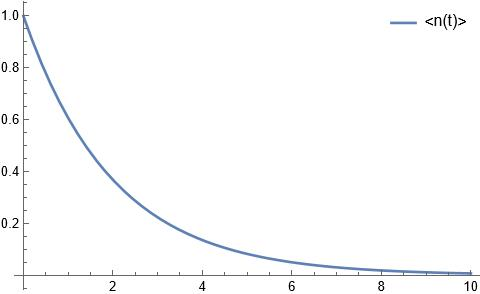
\includegraphics[width=0.6\linewidth]{NAnalitical.JPG}
	 	\caption{Average number of particles}
	 \end{figure}

	The evolution of the average number of particles is shown in Fig. \ref{fig:NAv}
	
	The same results for the average linear operators.
	
	We can also compare these results for the case when the higher order moments in Eq. \ref{eq:FinDinOfAv} are written out via Wick's theorem.
	
	\begin{figure}[h!]
		\begin{center}
			\begin{minipage}[h]{0.45\linewidth}
				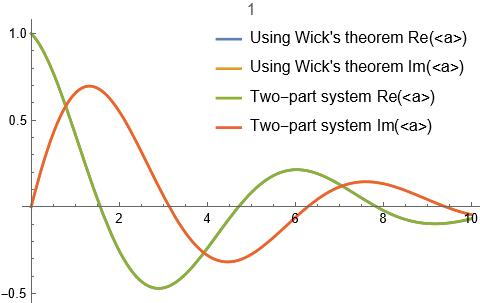
\includegraphics[width=1\linewidth]{Wickn0=1.JPG}
				\caption{Comparison with initial number of particles = 1}
				\label{fig:wick1}
			\end{minipage}
			\hfil
			\begin{minipage}[h]{0.45\linewidth}
				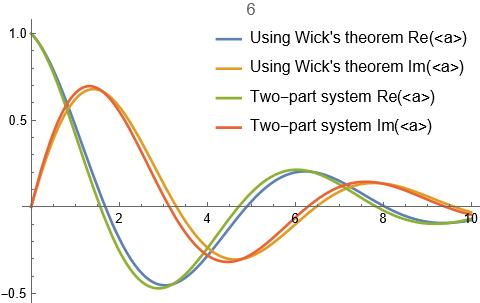
\includegraphics[width=1\linewidth]{Wickn0=6.JPG}
				\caption{Comparison with initial number of particles = 6}
				\label{fig:wick6}
			\end{minipage}
		\end{center}
	\end{figure}

	As can be seen in Fig. \ref{fig:wick1}, for the number of particles equal to 1, both methods give the same result, however, as the number of particles increases, they begin to decay, so the analytical results were obtained for two partial approximation and it stops working Fig. \ref{fig:wick6}.
	
	\section{Weak external field\label{sec:Efc}}
	
	In this section we consider the case when an external field is present in the system, i.e. $F \not= 0$. However, considering the general case is a difficult task due to the large number of summands in the oscillator, so we consider the case where the external field is small and the summands with $F^{1 + n}$, $n > 0$ can be neglected. 
	
	\begin{align}
		\label{eq:GenIntWithF}
		\mathcal{L}(t)\cdot &= -i\frac{\chi}{2}(({a^+}^2a^2\cdot) - (\cdot{a^+}^2a^2) + 2(e^{-\frac{\ga}{2}t} -1 ) [({a^+}a^2\cdot {a^+}) - (a\cdot{a^+}^2a) ] +2a_1^2b_2a_{21}({a^+}a^2\cdot) \nonumber\\
		&+ (2a_1^2b_2a_{22} - 2b_3a_3a_{42}^2)(a^2\cdot{a^+}) + 2b_1a_1 [a_{21}^2({a^+}^2a\cdot) + 2a_{21}a_{22}({a^+}a\cdot{a^+})] - 2a_3^2b_4a_{41}(\cdot{a^+}^2a) \\
		&+ (2b_1a_1a_{22}^2 - 2a_3^2b_4a_{42})(a\cdot{a^+}^2) - 2b_3a_3[a_{41}^2(\cdot{a^+}a^2) + 2 a_{41}a_{42}(a\cdot{a^+}a)) ]\nonumber,
	\end{align}
	where
	\begin{align*}
		a_1 &= e^{-\frac{\gamma  t}{4}+i \Delta  t}, \\
		b_1 &= \frac{F \left(4-4 e^{-\frac{\gamma  t}{4}+i \Delta  t}\right)}{\gamma -4 i \Delta },\\
		a_{21} &= e^{\frac{1}{4} t (\gamma -4 i \Delta )},\\
		a_{22} &= -2 e^{-i \Delta  t} \sinh \left(\frac{\gamma  t}{4}\right)\\
		b_2 &= \frac{F \left(4-4 e^{-\frac{1}{4} t (\gamma +4 i \Delta )}\right)}{\gamma +4 i \Delta },\\
		a_3 &= e^{-\frac{1}{4} t (\gamma +4 i \Delta )},\\
		b_3 &= \frac{F \left(4-4 e^{-\frac{1}{4} t (\gamma +4 i \Delta )}\right)}{\gamma +4 i \Delta },\\
		a_{41} &= e^{\frac{1}{4} t (\gamma +4 i \Delta )},\\
		a_{42} &= -2 e^{i \Delta  t} \sinh \left(\frac{\gamma  t}{4}\right),\\
		b_4 &= \frac{F \left(4-4 e^{-\frac{\gamma  t}{4}+i \Delta  t}\right)}{\gamma -4 i \Delta }.
	\end{align*}
	
	In this case, the action of the conjugate oscillator on an expression of type ${a^+}^na^m$ has the form
	
	\begin{align}
		\label{eq:ActOfGenOnExpr}
		\mathcal{L}^*(t){a^+}^na^m &= -i\frac{\chi}{2}(c_{00}{a^+}^na^m + c_{11}{a^+}^{n+1}a^{m+1} c_{01}{a^+}^na^{m + 1} + c_{12}{a^+}^{n + 1}a^{m + 2} \nonumber\\&+ c_{0-1}{a^+}^na^{m-1} + c_{-10}{a^+}^{n - 1}a^m + c_{10}{a^+}^{n+1}a^m + c_{21}{a^+}^{n+2}a^{m+1}),
	\end{align}
	where
	\begin{align*}
		c_{00} &= m (m-1)-n (n-1),\\
		c_{11} &= 2 (m-n) e^{\frac{1}{2} (-\gamma ) t},\\
		c_{01} &= 2 {a_1}^2 {a_{21}} {b_2} m-4 {a_3} {a_{41}} {b_3} n ({a_{41}}+{a_{42}}),\\
		c_{12} &= 2 {a_1}^2 {a_{21}} {b_2}+2 \left({a_1}^2 {a_{22}} {b_2}-{a_3} {a_{42}}^2 {b_3}\right)-2 {a_3} {a_{41}} {b_3} ({a_{41}}+2 {a_{42}}),\\
		c_{0-1} &= 2 {a_1} {a_{21}}^2 {b_1} m (m-1),\\
		c_{-10} &=-2 {a_3} {a_{41}}^2 {b_3} n (n-1),\\
		c_{10} &= 4 {a_1} {a_{21}} {b_1} m ({a_{21}}+{a_{22}})-2 {a_3}^2 {a_{41}} {b_4} n,\\
		c_{21} &= 2 {a_1} {a_{21}} {b_1} ({a_{21}}+2 {a_{22}})+2 \left({a_1} {a_{22}}^2 {b_1}-{a_3}^2 {a_{42}} {b_4}\right)-2 {a_3}^2 {a_41} {b_4}.
	\end{align*}
	As we see, in this case such operator does not give an identical 0 when acting on the particle number operator.
	
	
	
	\begin{figure}[h!]
		\begin{center}
			\begin{minipage}[h]{0.45\linewidth}
				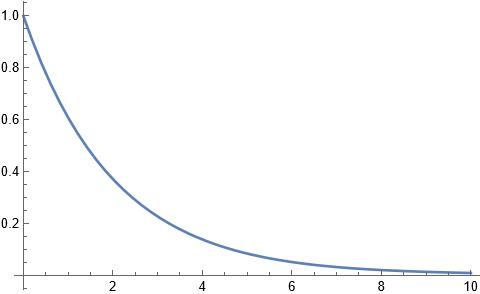
\includegraphics[width=1\linewidth]{NWeakForce.JPG}
				\caption{Average number of particles in the weak field}
				\label{fig:weakforcen}
			\end{minipage}
			\hfil
			\begin{minipage}[h]{0.45\linewidth}
				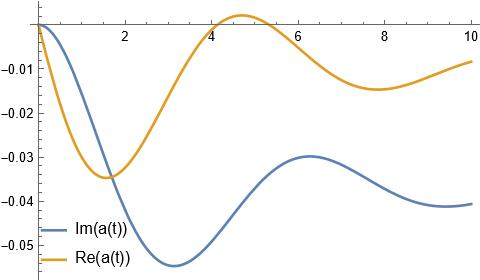
\includegraphics[width=1\linewidth]{aWeakForce.JPG}
				\caption{Mean of the linear operator in a weak field}
				\label{fig:weakforcea}
			\end{minipage}
			\hfil
			\begin{minipage}[h]{0.45\linewidth}
				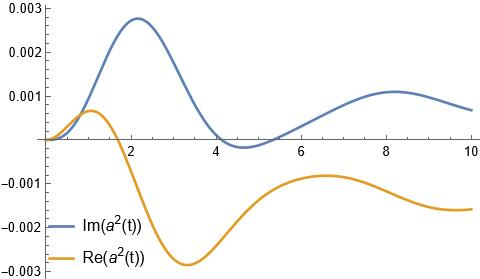
\includegraphics[width=1\linewidth]{a2WeakForce.JPG}
				\caption{Mean of the quadratic operator in a weak field}
				\label{fig:weakforceaa}
			\end{minipage}
		\end{center}
	\end{figure}
	
	We can also compare the difference of our method from the method of just using Wick's theorem in Eq. \ref{eq:FinDinOfAv}. This can be done by calculating our equation with $F = 0$. Once we have done this we can compare the results. The results are presented in Fig. \ref{fig:compn} \ref{fig:compa} \ref{fig:compa2}
	
	
	\begin{figure}[h!]
		\begin{center}
			\begin{minipage}[h!]{0.45\linewidth}
				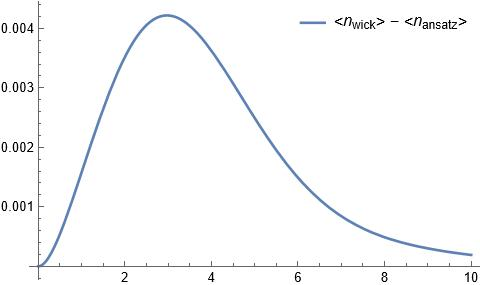
\includegraphics[width=1\linewidth]{Comparen.JPG}
				\caption{Comparison of results for average particle number}
				\label{fig:compn}
			\end{minipage}
			\hfil
			\begin{minipage}[h!]{0.45\linewidth}
				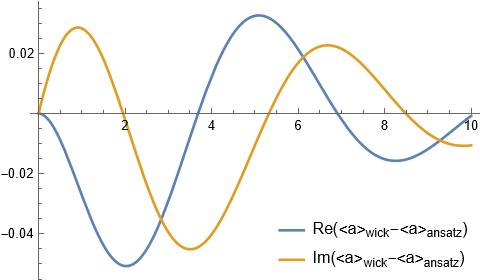
\includegraphics[width=1\linewidth]{Comparea.JPG}
				\caption{Comparison of results for Mean of the linear operator}
				\label{fig:compa}
			\end{minipage}
			\hfil
			\begin{minipage}[h!]{0.45\linewidth}
				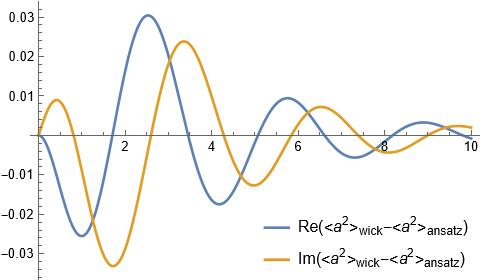
\includegraphics[width=1\linewidth]{Comparea2.JPG}
				\caption{Comparison of results for Mean of the quadratic operator}
				\label{fig:compa2}
			\end{minipage}
		\end{center}
	\end{figure}

	As can be seen, the results are of order $\la$, but for the mean quadratic operator the averages themselves are of the same order.
	
	
	
	\bibliographystyle{unsrt}
	\bibliography{ref}
	
%	\begin{thebibliography}{99}
		
%		\bibitem{KerrIntr} Lorenc D., Alpichshev Z. Dispersive effects in ultrafast nonlinear phenomena: The case of optical Kerr effect //Physical Review Research. – 2024. – V. 6. – N. 1. – Pg. 013042.
		
%		\bibitem{GaussState} Menu R., Roscilde T. Gaussian-state Ansatz for the non-equilibrium dynamics of quantum spin lattices //SciPost Physics. – 2023. – V. 14. – N. 6. – Pg. 151.
		
%		\bibitem{Kholevo} A.S. Kholevo Quantum systems, channels, information. M.: MCNMO, 2010.
		
%		\bibitem{MaslovN} Liu, Junqiu, et al. "High-yield, wafer-scale fabrication of ultralow-loss, dispersion-engineered silicon nitride photonic circuits." Nature communications 12.1 (2021): 2236.
		
%		\bibitem{MaslovSolve} S.P. Nikitin, A.V. Masalov. Quantum state evolution of the fundamental mode in the process of second-harmonic generation. Quantum Optics 3, № 2, 105-113 (1991).
		
%		\bibitem{Dis} Teretenkov A.E. (2018). Exactly solvable problems	irreversible quantum evolution
		
%		\bibitem{NosalTeretenkov} Nosal Iu.A., Teretenkov A.E.  "Higher order moments dynamics for some multimode quantum master equations." Lobachevskii Journal of Mathematics 43.7 (2022): 1726-1739.
		
%	\end{thebibliography}
	\newpage
	\section{Appendix\label{App}}
	
	\begin{theorem}
		\label{th:HeiGenerator}
		The generator $\mathcal{L}(t)\rho = -i[H_{\lambda},\rho] + \dfrac{\ga}{2}(a\rho a^+ - \dfrac12\{a^+a,\rho\}),$ in the Heisenberg representation has the form 
		\begin{equation*}
			\mathcal{L}^*\rho = i[H_{\la},\rho]  + \dfrac{\ga}{2}(a^+\rho a - \dfrac{1}{2}\{a^+a,\rho\}\}).
		\end{equation*}
	\end{theorem}
	
	\begin{demo}
		The operator $\mathcal{L}$ can be represented as $\mathcal{L} = \sum X_i\cdot Y_i$, then 
		
		\begin{equation*}
			\Tr(A\mathcal{L}B) = \sum\Tr(AX_i(B)Y_i)
		\end{equation*}
		
		Since the trace is invariant with respect to cyclic permutations, then 	
		
		\begin{equation*}
			\sum\Tr(AX_i(B) Y_i) = \sum\Tr(B Y_i(A)X_i) = \sum\Tr(B(Y_i\cdot X_i)(A)),
		\end{equation*}
		hence the operator $\mathcal{L}^*$ is represented in the form $\mathcal{L}^* = \sum Y_i \cdot X_i$
		
		
		The operator $\mathcal{L}$ can be rewritten as
		
		\begin{equation*}
			\mathcal{L}(B) = -i(HB\mathcal{I} - \mathcal{I}B H) + \dfrac{\ga}{2}(aB a^+ - \dfrac{1}{2}[a^+aB\mathcal{I} + \mathcal{I}B a^+a]),
		\end{equation*}
		hence
		
		\begin{equation*}
			Y(A)X = -iAH + iHA + \dfrac{\ga}{2}(a^+Aa - \dfrac{1}{2}[Aa^+a + a^+aA]),	
		\end{equation*}
		Thus we get the desired result.
	\end{demo}
	
	\begin{theorem}
		\label{th:DerOfGaus}
		The derivative of the Gaussian exponent can be expressed as a quadratic form
		
		\begin{equation*}
			\frac{d}{dt}\rho_{anz} = (\frac{1}{2}\mf{a}^TM\mf{a} + \mf{a}^TG + c)\rho_{anz},
		\end{equation*}
		where
		\begin{align*}
			M &= \frac{I}{C - \frac{J}{2}}\left(\frac{d}{dt}C\right)\frac{I}{C + \frac{J}{2}},\\
			G &= \left(  I + \frac{2I}{2J^{-1}C - I}  \right)\frac{d}{dt}\left(\frac{I}{C + \frac{J}{2}}m\right),\\
			c &=-m^T\frac{I}{2J^{-1}C -  I}\frac{d}{dt}\left(\frac{I}{C + \frac{J}{2}}m\right) + \frac{1}{2}\frac{d}{dt}m^T\left( \frac{I}{2J^{-1}C - I} - \frac{I}{2J^{-1}C + I} - KJ \right)J^{-1}m + \frac{d}{dt}c_t,
		\end{align*}
		where $g = -Km$, in which $m = (\braket{a} , \braket{a^+})^T$ and $C$ --- covariance matrix.
	\end{theorem}
	\begin{demo}
		The formula for the derivative of Gaussian ansatz can be found in \cite{Dis}
		\begin{equation}
			\label{eq:DerWithLin}
			\frac{d}{dt}\rho_{anz} = (\mf{a}^TM\mf{a} + \mf{a}^TG + c)\rho_{anz},
		\end{equation}
		where
		\begin{align*}
			M &= \frac{1}{2}\frac{I}{C - \frac{J}{2}}\left(\frac{d}{dt}C\right)\frac{I}{C + \frac{J}{2}},\\
			G &= e^{-KJ}\frac{d}{dt}\left(\frac{e^{KJ} - I}{KJ}g\right),\\
			c &= \frac{1}{2}g^TJ\frac{e^{-KJ} - I}{KJ}\frac{d}{dt}\left( \frac{e^{KJ} - I}{KJ}g  \right) + \frac{d}{dt}\left(  \frac{1}{2}g^T\frac{J}{KJ}(\text{sh}(KJ) - KJ)\frac{1}{KJ}g  +c_t \right).
		\end{align*}
		
		
			Using the formula $\text{arcoth}(x) = \frac{1}{2}\ln\left(\frac{x + 1}{x - 1}\right)$, we can explicitly write $e^{KJ}$.
		
		\begin{equation*}
			e^{KJ} = \frac{2J^{-1}C - I}{2J^{-1}C + I} = I - \frac{2I}{2J^{-1}C + I},
		\end{equation*}
		then
		\begin{align*}
			e^{-KJ}\frac{d}{dt}e^{KJ}J^{-1} =& -2\frac{2J^{-1}C + I}{2J^{-1}C - I}\frac{d}{dt}(2J^{-1}C + I)^{-1}J^{-1} = \\
			&4 \frac{2J^{-1}C + I}{2J^{-1}C - I} \frac{I}{2J^{-1}C + I}J^{-1}\left(\frac{d}{dt}C\right)\frac{I}{2J^{-1}C + I}J^{-1} = \\
			& 4 \frac{I}{2J^{-1}C - I}J^{-1}\left(\frac{d}{dt}C\right)\frac{I}{2J^{-1}C + I}J^{-1} = \frac{I}{C - \frac{J}{2}}\left(\frac{d}{dt}C\right)\frac{I}{C + \frac{J}{2}}
		\end{align*}
		
		In a similar way, we can simplify the vector $G$
		
		\begin{align*}
			G &= e^{-KJ}\frac{d}{dt}\left(\frac{e^{KJ} - I}{KJ}g\right) = \left(  I + \frac{2I}{2J^{-1}C - I}  \right)\frac{d}{dt}\left( \frac{
				\frac{2J^{-1}C - I}{2J^{-1}C + I} - I}{KJ}   g  \right) =\nonumber\\
			& = \left(  I + \frac{2I}{2J^{-1}C - I}  \right)\frac{d}{dt}\left( \frac{2I}{2J^{-1}C + I} J^{-1}m  \right) = \left(  I + \frac{2I}{2J^{-1}C - I}  \right)\frac{d}{dt}\left(\frac{I}{C + \frac{J}{2}}m\right).
		\end{align*}
		
		\begin{align*}
			&\frac{1}{2}g^TJ\frac{e^{-KJ} - I}{KJ}\frac{d}{dt}\left( \frac{e^{KJ} - I}{KJ}g  \right) = \frac{1}{2}g^TJ\frac{e^{-KJ} - I}{KJ}\frac{d}{dt}\left(\frac{I}{C + \frac{J}{2}}m\right) =\nonumber\\
			&=-\frac{1}{2}m^TKJ(KJ)^{-1}\left(I + 2\frac{I}{2J^{-1}C - I} - I\right)\frac{d}{dt}\left(\frac{I}{C + \frac{J}{2}}m\right) = -m^T\frac{I}{2J^{-1}C -  I}\frac{d}{dt}\left(\frac{I}{C + \frac{J}{2}}m\right)
		\end{align*}
		
		\begin{align*}
			\text{sh}(KJ) = \frac{I - \frac{2I}{2J^{-1}C + I} - I + \frac{2I}{2J^{-1}C - I}}{2} = \frac{I}{2J^{-1}C - I} - \frac{I}{2J^{-1}C + I}
		\end{align*}
		
		\begin{align*}
			&\frac{d}{dt}\left(  \frac{1}{2}g^TJ\frac{I}{KJ}(\text{sh}(KJ) - KJ)\frac{1}{KJ}g\right) = \frac{1}{2}\frac{d}{dt}m^T(\text{sh}(KJ) - KJ)J^{-1}m = \nonumber\\
			&\frac{1}{2}\frac{d}{dt}m^T\left( \frac{I}{2J^{-1}C - I} - \frac{I}{2J^{-1}C + I} - 2\text{arcoth}(-2J^{-1}C) \right)J^{-1}m
		\end{align*}
		
		\begin{align*}
			c = -m^T\frac{I}{2J^{-1}C -  I}\frac{d}{dt}\left(\frac{I}{C + \frac{J}{2}}m\right) + \frac{1}{2}\frac{d}{dt}m^T\left( \frac{I}{2J^{-1}C - I} - \frac{I}{2J^{-1}C + I} - KJ \right)J^{-1}m + \frac{d}{dt}c_t
		\end{align*}
		where
		
		\begin{equation}
			\label{eq:c}
			e^{c_t} = \left(\Tr e^{\frac{1}{2} \mathfrak{a}^TK\mathfrak{a} + g^T\mf{a}}\right)^{-1} = \sqrt{\left|\text{det}(e^{KJ} - I)\right|}e^{\frac{1}{2}g^TK^{-1}g}.
		\end{equation}
	\end{demo}
	
	\begin{theorem}
			\begin{equation*}
			\label{eq:RhoSq}
			\rho_{0,C}^2 = \frac{1}{\sqrt{|\det(2 C)|}} \rho_{0,C'}.
		\end{equation*}
		where 
		\begin{equation*}
			C' = - \frac{J}{4}\left(\frac{1}{2 J C} + 2 J C\right).
		\end{equation*}
	\end{theorem}
	\begin{demo}
		\begin{equation*}
			\rho_{0,C}^2 = \frac{Z'}{Z^2}\rho_{0,C'},
		\end{equation*}
		where 
		
		\begin{equation*}
			Z = \operatorname{tr} e^{\frac12 \mathfrak{a}^T K  \mathfrak{a}}  = \frac{1}{\sqrt{|\det(e^{KJ} - I)|}},
		\end{equation*}
		
		\begin{equation*}
			Z' = \operatorname{tr} e^{\frac12 \mathfrak{a}^T 2K  \mathfrak{a}}  = \frac{1}{\sqrt{|\det(e^{2KJ} - I)|}}.
		\end{equation*}
		
		Then 
		
		\begin{equation*}
			\frac{\operatorname{tr} e^{\frac12 \mathfrak{a}^T 2K  \mathfrak{a}}  }{(\operatorname{tr} e^{\frac12 \mathfrak{a}^T K  \mathfrak{a}})^2} = \sqrt{\left|\det\left(\frac{(e^{KJ} - I)^2}{e^{2 KJ} - I}\right)\right|}
		\end{equation*}
		
		\begin{equation*}
			\frac{(e^{KJ} - I)^2}{e^{2 KJ} - I} = \frac{e^{KJ} - I}{e^{KJ} + I} = \frac{1}{\coth \frac{KJ}{2}} = \frac{1}{-2J^{-1} C}
		\end{equation*}
		
		\begin{equation*}
			\frac{\operatorname{tr} e^{\frac12 \mathfrak{a}^T 2K  \mathfrak{a}}  }{(\operatorname{tr} e^{\frac12 \mathfrak{a}^T K  \mathfrak{a}})^2} = \sqrt{\left|\det\left(\frac{1}{-2J^{-1} C}\right)\right|} = \frac{1}{\sqrt{|\det(2 C)|}}
		\end{equation*}
	\end{demo}
\end{document} 